\documentclass[reprint,amsmath,amssymb,aps,pra,floatfix]{revtex4-2}
\usepackage{graphicx,bm,braket,hyperref,orcidlink,booktabs,placeins}
\hypersetup{hypertexnames=false,hidelinks}
\newtheorem{theorem}{Theorem}
\raggedbottom
\makeatletter
\setlength{\@fptop}{0pt}
\setlength{\@dblfptop}{0pt}
\makeatother
\begin{document}
\title{Finite-Instance Resource Certification for Group-Conditioned Discrimination of Huffman-Shaped Quantum Ensembles}
\author{Songyao Xue\,\orcidlink{0009-0009-5122-0963}}
\email{Contact author: 18637229290@139.com}
\affiliation{School of Software, Luoyang Normal University, No. 6 Jiqing Road, Yibin District, Luoyang, Henan Province, 471934, China}
\author{Mengsi Zhang\,\orcidlink{0009-0001-6793-9093}}
\thanks{These authors contributed equally to this work. Songyao Xue is listed first and Mengsi Zhang second.}
\affiliation{School of Artificial Intelligence, Dalian Maritime University, No. 1 Linghai Road, Ganjingzi District, Dalian City, Liaoning Province, 116026, China}
\date{}
\begin{abstract}
Nonuniform source statistics provide a structured way to allocate supports of quantum states in a common Hilbert space. We study group-conditioned minimum-error discrimination of Huffman-shaped ensembles, using classical Huffman lengths as source-dependent support-index parameters. The comparison is between a specified pair of encoders with the same source prior, ambient dimension, deterministic support-placement and amplitude--phase rules, group partition, orthogonal group side information, and conditional decoding model. Only the length vector differs. Resources are described by a support-index coordinate and a matched group-label coordinate. A primal-feasible grouped measurement for the Huffman ensemble and dual-feasible grouped operators for its matched fixed-length counterpart yield a sufficient finite-instance Pareto certificate. Huffman optimality orders the support-index coordinates, while a strictly positive primal-lower minus dual-upper gap orders the optimal measurement successes of the fixed ensemble pair. A pre-registered evaluation contains 220 rows, including seed replicas and trivial conditional tasks, with no post-selection of sources or partitions. Two distinct prior distributions in the registered $M=8$, $G=2$ probability-balanced setting satisfy the nontriviality gate and yield robust positive certificates, confirmed by repeat solves and independent full-space SDP validation. The result certifies specified finite instances within the declared constrained encoder family; its scope is pairwise discrimination, with the support index distinct from physical transmission cost.
\end{abstract}
\maketitle

\section{Introduction}
Nonuniform classical source statistics can influence the design of a finite quantum ensemble in two ways: through the prior probabilities used by the receiver and through the states assigned to the symbols. Classical prefix coding provides a well-defined allocation of integer lengths adapted to those statistics~\cite{shannon1948mathematical,huffman1952method,cover2006elements}. In quantum-state discrimination, the resulting source-weighted geometry determines the minimum-error measurement~\cite{helstrom1976quantum,holevo1973statistical,yuen1975optimum,barnett2009quantum,bae2015quantum}. This motivates the question of whether source-dependent support allocation can improve discrimination within a specified finite encoder architecture.

Quantum source coding includes asymptotic compression~\cite{schumacher1995quantum,jozsa1994new} and formulations with indeterminate or variable lengths~\cite{braunstein2000quantum,schumacher2001indeterminate,bostrom2002lossless,muller2009variable}. Coherent variable-length transmission involves length observables, termination, and decodability conditions. Here, classical Huffman lengths parameterize computational-basis supports of normalized states in a common ambient space. The operational task is one-shot minimum-error discrimination of this finite ensemble. The lengths supply support-index parameters rather than transmitted coherent codeword lengths.

An orthogonal group label supplies source-correlated side information and separates inter-group alternatives. Its availability changes the discrimination problem. A comparison between a labeled ensemble and an unlabeled reference therefore combines a change of payload geometry with a change of receiver information. We instead match the group partition, the orthogonal label alphabet, and its resource coordinate on both sides. The question is whether Huffman-shaped allocation improves success when the fixed-length counterpart receives exactly the same group side information.

The matched construction fixes the source prior, ambient Hilbert space, symbol ordering, cyclic support rule, equal-modulus amplitudes, deterministic phases, and conditional measurement model. The Huffman and fixed-length arms differ only in their length vectors. Each arm consequently produces one specified ensemble, whose measurement success can be bounded by semidefinite programming (SDP)~\cite{eldar2003designing,watrous2018theory,boyd2004convex}. The resource vector records the average support index and ideal group-label width separately, avoiding a scalar exchange rate between heterogeneous coordinates.

The contributions are threefold. First, we formulate this matched constrained encoder comparison explicitly. Second, we prove a primal--dual finite-instance Pareto certificate: a feasible Huffman grouped measurement lower bound exceeding a feasible matched fixed-length grouped dual upper bound implies strict success improvement without a larger support index or label width. Third, a pre-registered evaluation of outcome-independent grouping rules identifies robust positive probability-balanced cases, with all registered rows reported and two distinct priors independently validated. The numerical diagnostics and Supplemental Material~\cite{supplemental_material} provide finite-instance tests of this result.

The certificate concerns optimal measurements for the specified encoder pair, with the partition held fixed. Unrestricted fixed-length encoder classes can admit mutually orthogonal states and unit success. The constrained architecture, explicit information matching, and finite-instance evidence determine the scope of the comparison. Scalable approximate-decoder diagnostics and effective logical-noise models are secondary extensions. Table~\ref{tab:notation} summarizes the main notation.

\section{Operational Model and Huffman-Shaped Ensembles}
\label{sec:model}
\subsection{Source and common ambient space}
Let the source alphabet be $\{s_i\}_{i=0}^{M-1}$, with $M\ge2$, positive priors $p_i$, and $\sum_i p_i=1$. Let $l_i^H$ be binary Huffman lengths, and define
\begin{equation}
 n_{\rm fix}=\lceil\log_2 M\rceil,\qquad l_i^F=n_{\rm fix}.
 \label{eq:lengths}
\end{equation}
Both arms $X\in\{H,F\}$ use the same space
\begin{equation}
 \mathcal H_{\max}=(\mathbb C^2)^{\otimes n_{\max}},\quad
 n_{\max}=\max\{n_{\rm fix},\max_i l_i^H\}+1,
 \label{eq:ambient}
\end{equation}
of dimension $d=2^{n_{\max}}$. The support size associated with length $l_i^X$ is
\begin{equation}
 b_i^X=2^{n_{\max}-l_i^X}.
 \label{eq:support-size}
\end{equation}
These integers specify the encoder's support allocation. The ambient dimension is shared even when the two length vectors differ.

\begin{table*}[tbp]
\caption{Notation for the matched comparison. A star denotes measurement optimization for a fixed ensemble and partition.}
\label{tab:notation}
\centering\small
\begin{tabular}{@{}p{0.17\textwidth}p{0.77\textwidth}@{}}
\toprule
\textbf{Symbol} & \textbf{Meaning}\\
\midrule
$M,s_i,p_i$ & Alphabet size, zero-based source symbol, and positive normalized prior.\\
$l_i^H,l_i^F,n_{\rm fix}$ & Huffman support index, fixed support index, and $\lceil\log_2M\rceil$.\\
$n_{\max},d,\mathcal H_{\max}$ & Common ambient qubit index, dimension $2^{n_{\max}}$, and Hilbert space.\\
$\mathcal A,S_i^X,b_i^X$ & Matched deterministic encoder, assigned support, and support cardinality ($X=H,F$).\\
$\ket{\Phi_i^X},\rho_i^X,\Gamma_{ij}^X$ & Payload state, its density operator, and inner product $\braket{\Phi_i^X|\Phi_j^X}$.\\
$g(i),\mathcal G_g,G$ & Common group map, group members, and number of groups.\\
$p_g,q_i^{(g)},\ket{a_g}$ & Group probability, conditional prior $p_i/p_g$, and orthogonal group label.\\
$E_i^{X,g},Y_g^F$ & Conditional POVM effect and fixed-arm dual feasible operator.\\
$P_X^*,\underline P_H,\overline P_F$ & Optimal conditional measurement success, H primal lower bound, and F dual upper bound.\\
$\Delta_{\rm pair}$ & Certificate gap $\underline P_H-\overline P_F$.\\
$C_L^X,C_A,\mathbf C_X$ & Support-index coordinate, matched label width $\lceil\log_2G\rceil$, and resource vector.\\
$\epsilon_{\rm orth},\epsilon_{\rm SDP}$ & Numerical orthogonality threshold and solver tolerance.\\
\bottomrule
\end{tabular}
\end{table*}

\subsection{Matched deterministic encoder}
\label{sec:encoder}
The architecture $\mathcal A$ assigns supports by decreasing prior probability, using the frozen implementation's ordering for ties. With a cyclic cursor $c$ initially zero, the symbol $i$ encountered next receives
\begin{equation}
 S_i^X=\{(c+k)\bmod d:0\le k<b_i^X\},
 \label{eq:support-rule}
\end{equation}
after which $c$ advances by $\max\{1,b_i^X/2\}$ modulo $d$. Each support is sorted in increasing computational-basis order. The rule is executed separately for each length vector with the same initial cursor. The shift parameter is zero on both arms. Support overlap is determined by this rule rather than independently optimized.

Write $x_{i,k}^X$ for the $k$th element of the sorted support, with $0\le k<b_i^X$. The payload is
\begin{equation}
 \ket{\Phi_i^X}=\frac{1}{\sqrt{b_i^X}}
 \sum_{k=0}^{b_i^X-1} e^{i\theta_{i,k}^X}\ket{x_{i,k}^X},
 \label{eq:payload}
\end{equation}
where the existing deterministic phase construction is
\begin{equation}
 \theta_{i,k}^X=\frac{2\pi(i+1)(k+1)}{b_i^X+1}\pmod{2\pi}.
 \label{eq:phase}
\end{equation}
The architecture has zero optimizer iterations and makes no random amplitude or phase draws. Both arms share the source-seed policy; the deterministic mode makes the encoder independent of that seed once the prior is fixed. Define $\rho_i^X=\ket{\Phi_i^X}\bra{\Phi_i^X}$. The only systematic input difference is $l^H$ versus $l^F$; the differing supports and phases are consequences of the same formulas.

\subsection{Support-index resource ordering}
The declared resource vector is
\begin{equation}
 \mathbf C_X=(C_L^X,C_A),\quad
 C_L^H=\bar L_H=\sum_i p_i l_i^H,\quad C_L^F=n_{\rm fix}.
 \label{eq:resource-vector}
\end{equation}
The coordinate $C_L$ is a length-derived support index: smaller lengths permit larger supports in Eq.~\eqref{eq:support-size}. It is distinct from support cardinality, physical qubit count, and communication cost. The shared physical ambient width is $n_{\max}$, not $\bar L_H$. A smaller $C_L$ therefore expresses an ordering in this declared model, not a reduction of the state-preparation dimension.

An $M$-word binary code with constant length $n_{\rm fix}$ is prefix feasible because $M2^{-n_{\rm fix}}\le1$. Huffman optimality among binary prefix codes~\cite{huffman1952method,cover2006elements} gives
\begin{equation}
 \bar L_H\le n_{\rm fix}.
 \label{eq:length-order}
\end{equation}
The argument applies to non-power-of-two alphabets and probability ties. Positivity of the priors and $M\ge2$ exclude unused symbols and the single-symbol length convention.

\section{Matched Group-Conditioned Discrimination}
\label{sec:group}
\subsection{Common side information}
Fix a partition $\{\mathcal G_g\}_{g=0}^{G-1}$ and its map $g(i)$. Both arms use the same orthonormal labels $\{\ket{a_g}\}$ and states
\begin{equation}
 \ket{\Psi_i^X}=\ket{\Phi_i^X}\otimes\ket{a_{g(i)}},\qquad
 C_A=\lceil\log_2G\rceil.
 \label{eq:labels}
\end{equation}
The label contains source-correlated side information. Its ideal register-width coordinate is charged identically to both arms. This coordinate excludes architecture-specific preparation and readout costs, which require an additional operational model.

The label measurement identifies $g$ without error in this ideal model. Set
\begin{equation}
 p_g=\sum_{i\in\mathcal G_g}p_i,\qquad
 q_i^{(g)}=p_i/p_g.
 \label{eq:conditional-prior}
\end{equation}
Positive source priors and nonempty groups give $p_g>0$. A conditional positive-operator-valued measure (POVM) has effects $E_i^{X,g}\succeq0$ satisfying $\sum_{i\in\mathcal G_g}E_i^{X,g}=I$ on $\mathcal H_{\max}$. Its success is
\begin{equation}
 P_X(E)=\sum_g p_g\sum_{i\in\mathcal G_g}q_i^{(g)}
       \operatorname{Tr}(E_i^{X,g}\rho_i^X).
 \label{eq:success}
\end{equation}
Let $P_X^*$ denote the maximum of Eq.~\eqref{eq:success} for the fixed states and partition. This optimization changes measurements, while the encoder architecture, support placement, phases, and group map remain fixed.

\begin{figure*}[tbp]
\centering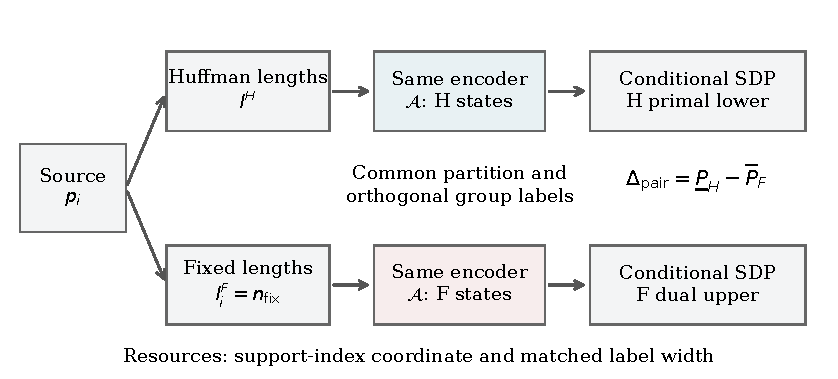
\includegraphics[width=\textwidth]{figures/matched_operational_model.pdf}
\caption{Matched operational comparison. The two length vectors enter the same deterministic encoder in the same ambient space. A common partition and identical orthogonal group labels define both conditional discrimination tasks. The certificate compares an H primal lower bound with an F grouped dual upper bound.}
\label{fig:model}
\end{figure*}

\subsection{Outcome-independent partitions}
Four rules fix the partition before any SDP result. G0 uses one group. G1 assigns zero-based indices by $g(i)=i\bmod G$. G2 sorts symbols by $(-p_i,i)$ and assigns each to the group with least accumulated probability, breaking mass ties by group index. G3 cuts the classical Huffman tree into $G$ subtrees: starting with the root, it splits the shallowest nonleaf frontier node, with ties resolved by minimum leaf index and then node serial. The same resulting partition is applied to both payload ensembles. The exact tree tie-breaking and source seed lists are provided in the Supplemental Material~\cite{supplemental_material}.

G1 uses only indices; G2 uses only priors; G3 uses only classical tree topology. None uses quantum overlap, SDP success, or certificate sign. Overlap-aware partitioning belongs to secondary heuristic diagnostics rather than this matched registered comparison.

\section{Matched Finite-Instance Pareto Certificate}
\label{sec:certificate}
For each group, feasible H effects yield
\begin{equation}
 \underline P_H=\sum_g p_g\sum_{i\in\mathcal G_g}q_i^{(g)}
     \operatorname{Tr}(E_i^{H,g}\rho_i^H)\le P_H^*.
 \label{eq:lower}
\end{equation}
The matched F dual consists of Hermitian operators satisfying
\begin{equation}
 Y_g^F\succeq q_i^{(g)}\rho_i^F\quad(i\in\mathcal G_g),\qquad
 \overline P_F=\sum_g p_g\operatorname{Tr}Y_g^F.
 \label{eq:dual}
\end{equation}
Groupwise weak duality implies $P_F^*\le\overline P_F$. In particular, an ungrouped F dual is not the dual for this side-information-matched task.

\begin{theorem}[Matched Pareto certificate]
\label{thm:main}
Fix positive normalized priors $p$, a common ambient Hilbert space, and a constrained encoder architecture $\mathcal A$ with the same generation rules, seed policy, and optimization protocol for both arms. Let H use binary Huffman lengths and F use $l_i^F=n_{\rm fix}=\lceil\log_2 M\rceil$. Fix the same partition, orthogonal group-label alphabet, label coordinate $C_A$, and conditional POVM decoding model for both output ensembles. Suppose $\underline P_H$ is obtained from primal-feasible grouped H effects and $\overline P_F$ from dual-feasible grouped F operators as in Eqs.~\eqref{eq:lower} and \eqref{eq:dual}. If
\begin{equation}
 \Delta_{\rm pair}=\underline P_H-\overline P_F>0,
 \label{eq:certificate}
\end{equation}
then $P_H^*>P_F^*$, $\bar L_H\le n_{\rm fix}$, and $C_A^H=C_A^F$. For this specified encoder pair, H strictly Pareto-dominates F in the ordering that maximizes success and minimizes the support-index and label coordinates.
\end{theorem}

\textit{Proof.} Feasible H effects give $P_H^*\ge\underline P_H$. For any feasible F effects in group $g$, dual feasibility and positivity imply
\begin{align}
 \sum_{i\in\mathcal G_g}q_i^{(g)}\operatorname{Tr}(E_i^{F,g}\rho_i^F)
 &\le\sum_{i\in\mathcal G_g}\operatorname{Tr}(E_i^{F,g}Y_g^F)\nonumber\\
 &=\operatorname{Tr}Y_g^F.
\end{align}
Multiplication by the positive $p_g$ and summation over groups yield $P_F^*\le\overline P_F$. Thus Eq.~\eqref{eq:certificate} implies
\begin{equation}
 P_H^*\ge\underline P_H>\overline P_F\ge P_F^*.
\end{equation}
Huffman optimality gives Eq.~\eqref{eq:length-order}; the common label alphabet gives equal $C_A$. In minimization form, the objective vectors are $(\bar L_H,C_A,-P_H^*)$ and $(n_{\rm fix},C_A,-P_F^*)$. The former is no larger in any coordinate and strictly smaller in success's negative coordinate. This is Pareto dominance with at least one strict improvement, including when $\bar L_H=n_{\rm fix}$. \(\square\)

The theorem is an exact implication from feasibility. Its numerical application uses postprocessed floating-point operators and reported residuals; it is not an interval-arithmetic proof. A nonpositive gap leaves this sufficient test inconclusive. No scalar resource exchange rate enters the theorem.

\begin{figure}[tbp]
\centering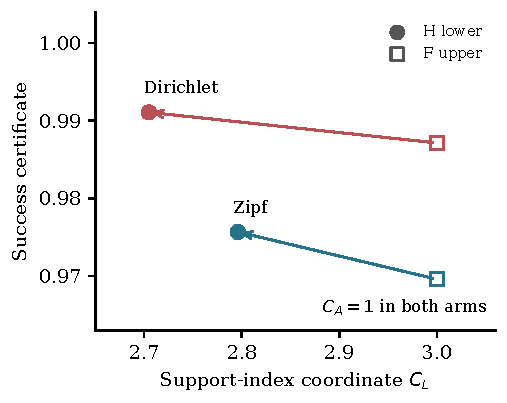
\includegraphics[width=\columnwidth]{figures/pareto_coordinates.pdf}
\caption{Certificate-based resource ordering for the two validated G2 priors. Filled circles are H lower bounds; open squares are F upper bounds. Leftward and upward movement improves the declared support-index/success ordering, with $C_A=1$ held equal. The axes express model coordinates and numerical bounds, not physical transmission savings.}
\label{fig:pareto}
\end{figure}

\section{Pre-Registered Finite-Instance SDP Evidence}
\subsection{Evaluation protocol and counting}
\label{sec:protocol}
The registry was frozen before evaluation. It contains $M=4,8$ and near-uniform, Zipf, Dirichlet, and strong-skew families, with five source seeds per family and alphabet size. The 40 registered source entries represent 24 distinct prior vectors because Zipf and strong-skew priors are seed-independent at fixed parameters. Each source is evaluated under G0 with $G=1$; G1--G3 use $G=2$ for $M=4$ and $G=2,4$ for $M=8$. This gives 220 registered rows. A row is a source-entry/rule/group-count configuration, not an independent prior draw.

Both arms use Sec.~\ref{sec:encoder}'s deterministic architecture and the same partition. Conditional primal and dual SDPs are solved with SCS through CVXPY~\cite{diamond2016cvxpy,agrawal2018rewriting}, using $\epsilon_{\rm SDP}=5\times10^{-6}$, at most 25000 iterations, and a 30-s time limit per solve. State-span compression is followed by ambient-space lifting, primal repair, and a dual safety shift. Feasibility is checked in the original space at tolerance $10^{-7}$. The pre-registered robust-positive criterion is
\begin{equation}
 \Delta_{\rm pair}>100\epsilon_{\rm SDP}=5\times10^{-4}.
 \label{eq:robust}
\end{equation}
All 220 rows, including fixed-trivial and nonpositive cases, are reported. Sources, partitions, group counts, encoder settings, and the threshold were fixed without certificate-based selection. Every robust-positive row was re-solved and independently checked in the full ambient space. Seed replicas provide reproducibility checks rather than additional independent priors.

\subsection{Conditional-task nontriviality}
\label{sec:nontriviality}
For arm $X$, let $\Gamma_{ij}^X=\braket{\Phi_i^X|\Phi_j^X}$. A group is numerically nontrivial when it has at least two members and
\begin{equation}
 \max_{i\ne j\in\mathcal G_g}|\Gamma_{ij}^X|>
 \epsilon_{\rm orth}=10^{-10}.
 \label{eq:nontrivial}
\end{equation}
Matched E1 means at least one common positive-mass group is nontrivial in both arms. Matched E2 means at least one nonsingleton group exists and every nonsingleton group is nontrivial in both arms. Singletons are reported separately and excluded from E2's universal quantifier. These diagnostics are computed before solving the SDPs. The classifications agree with a $10^{-8}$ sensitivity threshold.

All G0 tasks are globally nontrivial in both arms. Pooled fixed-trivial rates are $0.60$ for G1, $0.08333$ for G2, and zero for G3. Of all registered rows, 179 satisfy matched E1 and 138 matched E2; 41 have a fixed-trivial conditional task. Here fixed-trivial denotes within-group orthogonality at the stated numerical threshold. G2 and G3 preserve nontrivial F conditional tasks more frequently than G1 in this sample. Table~\ref{tab:registered} resolves the rates by $M$ and $G$, and Fig.~\ref{fig:nontriviality} gives the pooled diagnostics.
\begin{table*}[tbp]
\caption{Pre-registered matched-certificate summary. Counts include all rows, including seed replicas, singleton groups, and fixed-trivial tasks. Distinct positive priors are deduplicated within each cell; the same prior can occur in different cells. E1 and E2 are defined in Sec.~\ref{sec:nontriviality}.}
\label{tab:registered}
\centering\small
\begin{tabular}{@{}lrrrrrrr r@{}}
\toprule
\textbf{Rule} & $M$ & $G$ & \textbf{Rows} & \textbf{Fixed-trivial} & \textbf{E1} & \textbf{E2} & \textbf{Robust-positive} & \textbf{Positive priors} \\
\midrule
G0 & 4 & 1 & 20 & 0.00 & 20 & 20 & 0 & 0 \\
G0 & 8 & 1 & 20 & 0.00 & 20 & 20 & 0 & 0 \\
G1 & 4 & 2 & 20 & 0.55 & 9 & 4 & 0 & 0 \\
G1 & 8 & 2 & 20 & 0.50 & 10 & 8 & 0 & 0 \\
G1 & 8 & 4 & 20 & 0.75 & 5 & 0 & 0 & 0 \\
G2 & 4 & 2 & 20 & 0.00 & 20 & 11 & 1 & 1 \\
G2 & 8 & 2 & 20 & 0.00 & 20 & 15 & 6 & 2 \\
G2 & 8 & 4 & 20 & 0.25 & 15 & 0 & 0 & 0 \\
G3 & 4 & 2 & 20 & 0.00 & 20 & 20 & 1 & 1 \\
G3 & 8 & 2 & 20 & 0.00 & 20 & 20 & 0 & 0 \\
G3 & 8 & 4 & 20 & 0.00 & 20 & 20 & 0 & 0 \\
\bottomrule
\end{tabular}
\end{table*}

\begin{figure*}[tbp]
\centering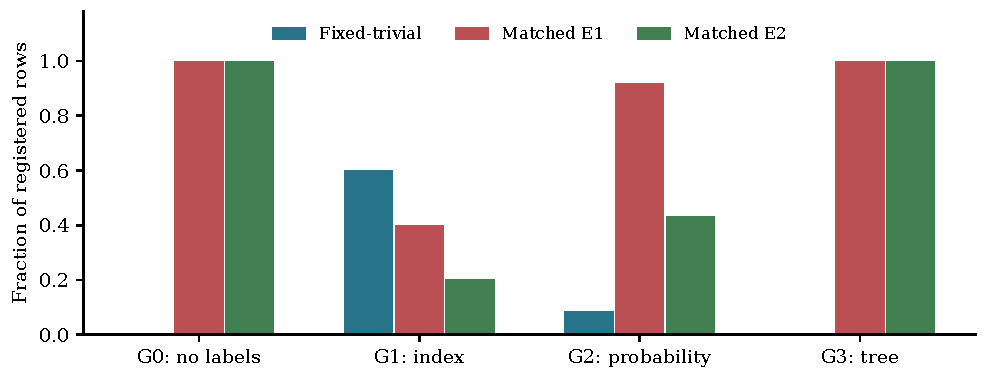
\includegraphics[width=\textwidth]{figures/grouping_nontriviality.pdf}
\caption{Conditional nontriviality over every registered row. Rates are pooled within each rule: G0 has 40 rows and each of G1--G3 has 60. E1 and E2 use the matched definitions in Sec.~\ref{sec:nontriviality}; their denominators include fixed-trivial rows and singleton-containing partitions.}
\label{fig:nontriviality}
\end{figure*}

\subsection{Pairwise certificates across grouping rules}
\label{sec:all-results}
All 220 certificate pairs pass the numerical feasibility checks. Across 1040 conditional certificate sets, the largest H primal residual is $1.21\times10^{-14}$ and the recorded F dual violation is zero. Figure~\ref{fig:gaps} shows every registered gap. Robust-positive row counts are zero for G0, zero for G1, seven for G2, and one for G3. The G2 count comprises six $M=8,G=2$ rows and one $M=4,G=2$ row. These seven rows involve seven registered source entries and three distinct priors. The G3 positive uses the same $M=4$ prior as the G2 positive there; it supplies additional pre-registered evidence but only one prior for that rule.

No robust positive pairwise certificate was observed for the registered $G=1$ cases. This records the absence of a satisfied sufficient certificate in the sample, rather than a general success ordering. Fixed-trivial, zero, and negative cases remain in the accounting. The row counts describe the fixed evaluation matrix and do not estimate population probabilities of advantage.

\begin{figure*}[tbp]
\centering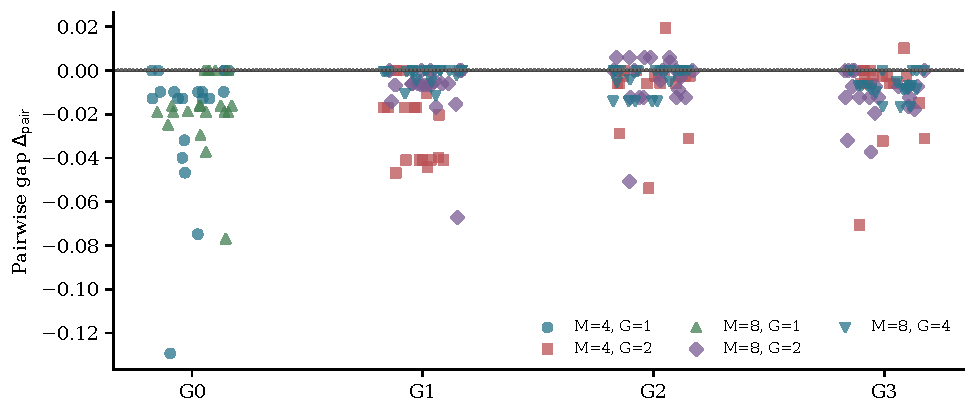
\includegraphics[width=\textwidth]{figures/all_certificate_gaps.pdf}
\caption{All 220 registered pairwise gaps, including nonpositive and fixed-trivial cases. Horizontal offsets distinguish overlapping rows without changing gap values. The solid line is zero; the dotted line is the pre-registered robust-positive threshold $5\times10^{-4}$. Marker types distinguish alphabet size and group count. Seed replicas are plotted as separate registered rows.}
\label{fig:gaps}
\end{figure*}

\subsection{Two validated probability-balanced priors}
\label{sec:validated}
The $M=8,G=2$ G2 cell has 20 registered rows, of which 15 satisfy matched E2 and six have robust positive certificates. Those six rows represent six registered source entries but only two distinct prior vectors: five seed entries share the Zipf prior and one is a Dirichlet draw. Both distinct priors pass E2, repeat solving, and independent full-space SDP validation. Table~\ref{tab:validated} gives their priors, lengths, common partitions, resource coordinates, bounds, and residuals.

The registered gaps are $0.006090$ for Zipf and $0.003941$ for Dirichlet after rounding. Independent full-space solves yield gaps $0.006025$ and $0.003776$, respectively, each exceeding Eq.~\eqref{eq:robust}'s threshold. The distinct stored prior vectors establish prior-level evidence; the repeated Zipf seeds establish repeatability of one prior. Figure~\ref{fig:validated} compares the H lower and F upper bounds for both solver formulations.
\begin{table*}[tbp]
\caption{Two distinct validated G2 priors with $M=8$, $G=2$, and matched E2 tasks. Symbols and partitions use zero-based indices. Bounds and residuals are registered values; the final two rows give the independent ambient-space re-solve. Prior vectors are displayed to four decimals; certificates use the full-precision stored priors.}
\label{tab:validated}
\centering\small
\begin{tabular}{@{}lcc@{}}
\toprule
\textbf{Quantity} & \textbf{Zipf} ($s=0.8$) & \textbf{Dirichlet} ($\alpha=2$) \\
\midrule
Source seed & 51808 & 2837 \\
$(p_0,\ldots,p_3)$ & $(0.3092,0.1776,0.1284,0.1020)$ & $(0.0477,0.0211,0.0644,0.1103)$ \\
$(p_4,\ldots,p_7)$ & $(0.0853,0.0737,0.0652,0.0586)$ & $(0.2621,0.1018,0.1576,0.2350)$ \\
Huffman length vector & $(2,2,3,3,4,4,4,4)$ & $(5,5,4,3,2,3,3,2)$ \\
Group $0$ & $\{0,4,5,7\}$ & $\{1,3,4,5\}$ \\
Group $1$ & $\{1,2,3,6\}$ & $\{0,2,6,7\}$ \\
$\bar L_H$ & 2.796049 & 2.704828 \\
$n_{\rm fix}$ & 3 & 3 \\
$n_{\max}$ & 5 & 6 \\
$C_A$ (both arms) & 1 & 1 \\
$\underline P_H$ & 0.975660 & 0.991066 \\
$\overline P_F$ & 0.969570 & 0.987125 \\
$\Delta_{\rm pair}$ & 0.006090 & 0.003941 \\
H primal residual & 6.96e-15 & 1.20e-14 \\
F dual violation & 0.0 & 0.0 \\
Repeat solve / full-space check & PASS / PASS & PASS / PASS \\
Full-space H lower / F upper & 0.975645 / 0.969620 & 0.991062 / 0.987286 \\
Full-space certificate gap & 0.006025 & 0.003776 \\
\bottomrule
\end{tabular}
\end{table*}

\begin{figure*}[tbp]
\centering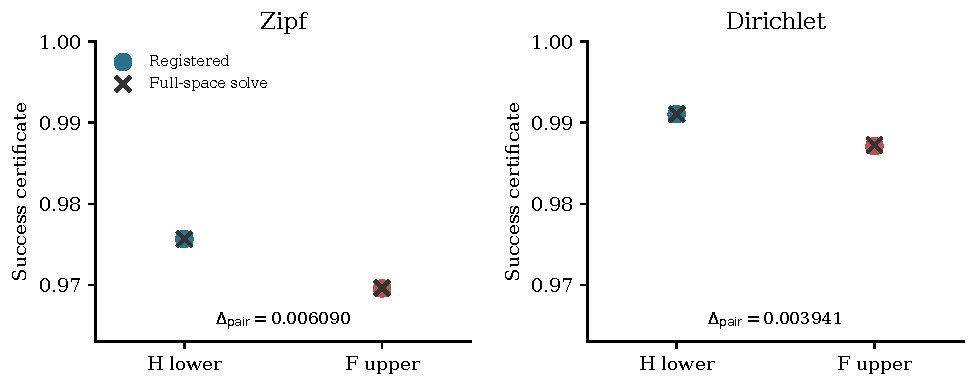
\includegraphics[width=\textwidth]{figures/validated_g2_priors.pdf}
\caption{The two distinct G2 positive priors with $M=8,G=2$ and E2 nontriviality. Filled markers show registered H lower and F upper bounds; crosses show the independent ambient-space re-solve. Each pair has a positive certified success separation at equal label width and no greater H support index. These are two prior vectors, not six independent draws.}
\label{fig:validated}
\end{figure*}

\onecolumngrid
\clearpage
\twocolumngrid
\section{Extensions and Limitations}
Matching side information isolates the allocation comparison: each receiver knows the same group, and the corresponding F upper bound is itself grouped. Thus the certificate does not attribute the mere availability of additional label information to Huffman shaping. Label width is an explicit equal resource coordinate; implementing that information physically requires further preparation and readout accounting.

The encoder family fixes support placement, equal-modulus amplitudes, deterministic phases, and generation effort. In the unrestricted fixed-length support class, individual basis states can realize mutually orthogonal encodings in this ambient space, attaining unit success. That optimization problem is distinct from the specified-pair comparison. The present certificate concerns measurement optima for the two fixed output ensembles. Broader encoder optimization and independently optimized partitions require their own matched comparisons.

The support-index coordinate expresses the classical allocation rule, while success is operational for the ideal labeled discrimination task. The Pareto ordering consequently has model-specific resource semantics. Finite numerical certificates additionally depend on feasibility postprocessing and floating-point residual checks. Formal interval-certified arithmetic would strengthen numerical rigor. The positive cases establish the stated sufficient inequality for two validated priors, without a universal allocation or grouping ordering.

Quantum error correction (QEC), represented by an effective logical-failure model, and maximum-a-posteriori (MAP) post-processing can extend the decoding task by adding a recovered-channel model and a posterior decision rule~\cite{nielsen2010quantum,terhal2015quantum,berger1985statistical}. Their syndrome, fallback, and reliability details are provided in the Supplemental Material~\cite{supplemental_material}; they are modular extensions, not inputs to Theorem~\ref{thm:main}. Architecture-specific fault-tolerant costs remain a separate physical-model question.

The pretty-good measurement (PGM)~\cite{hausladen1994pretty,eldar2001quantum} supplies scalable approximate-decoder diagnostics. The Supplemental Material contains the PGM sweeps, scalarized efficiency and weighted-cost sensitivity analyses, effective QEC reliability curves, and bounded-overlap surrogate conditions. Their evidential role is secondary and convention dependent; the main comparison uses grouped primal and dual SDP certificates and the resource vector in Eq.~\eqref{eq:resource-vector}.

\section{Conclusion}
Huffman lengths define source-dependent support-index allocations within a fixed deterministic quantum encoder. Matching the partition and orthogonal group side information on both arms yields a conditional discrimination comparison in which only the length-vector input changes. A feasible grouped H measurement and a feasible grouped F dual operator certify strict success improvement for a specified pair whenever their aggregated bounds separate. Huffman optimality and equal label width then give a pairwise Pareto ordering in the declared support-index resource model.

The pre-registered evaluation reports all 220 rows and identifies two distinct validated positive priors in the probability-balanced $M=8,G=2$ setting. These finite-instance results are constrained-encoder certificates rather than a universal advantage over fixed-length encodings. Broader matched encoder families and larger confirmatory SDP studies are natural next steps; architecture-specific noise and hardware accounting require additional models.

\FloatBarrier
\section*{Data availability}
The data and code for the secondary analyses are publicly archived in Ref.~\cite{xue_zhang_zenodo_2026}, Version 1.0.0. The registered matched-comparison data, stored certificate operators, and reproducibility protocols accompany this manuscript in the Supplemental Material~\cite{supplemental_material}. The archive DOI identifies the frozen earlier release, not the additional registered data.
\bibliographystyle{apsrev4-2}
\bibliography{references}
\end{document}
